\chapter{Implémentation}
\label{ch:impl}

\section{Choix d'implémentations}
\subsection{Langage}
Au départ le choix du langage s'est porté sur sagemath (framework python) afin de mieux comprendre les différents calculs et faire un premier POC du chiffrement.
Cependant l'implémentation du POC était lente et le changement d'algorithme pour les pairings était difficile.
Je me suis donc orienté sur le C pour avoir de meilleures performances et pouvoir mieux gérer ma mémoire car c'est un point important dans des logiciels implémentant de la cryptographie. Pour pouvoir faire facilement des calculs sur les courbes elliptiques et les pairings en C il me fallait une librairie.

\begin{table}[h!]
	\centering
	\begin{tabular}{ |p{3cm}||p{3cm}|p{3cm}| }
		\hline
		\multicolumn{3}{|c|}{Temps des algorithmes entres langages [s]} \\
		\hline
		Algorithms& C &Sage\\
		\hline
		Setup   & 0.2856898 & 6.5858234\\
		Encrypt & 0.0061584 & 7.6450206\\
		Decrypt & 0.00951 & 3.3274426\\
		\hline
	\end{tabular}
\caption{Table de comparaison des temps d'exécution pour les différents algorithmes de Certificateless Cryptography }
\label{table:comparisonTimeAlgo}
\end{table}

\subsection{Librairie cryptographique}
%TODO + d'explications sur les librairies et les choix faits (retrouver l'endoit où l'on dit que RELIC est plus efficient et est plus fait pour les POCs etc)
La librairie utilisée est RELIC Toolkit~\cite{relic-toolkit}, c'est une librairie en cours de développement qui se veut efficiente. Sa concurrence avec MIRACL m'a fait hésiter dans mon choix, mais MIRACL est plus codée en~ C++ avec des équivalences en C j'ai donc choisi RELIC. De plus j'ai trouvé par exemple ici~\cite{bibid} que RELIC était généralement plus adapté dans le domaine universitaire pour des POC 
\subsection{Courbe utilisée}
La courbe utilisée pour le POC est la BLS12-P381, en effet cette courbe est assez efficiente et compatible avec les pairings. De plus RELIC l'a dans ses options et fonctionne bien, elle a un niveau de sécurité de 128bits. Je voulais prendre une courbe avec une plus grande sécurité cependant RELIC ne l'a pas encore totalement implémenté (certains tests concernant $\mathbb{G}_2$ ne passes pas), mais la librairie étant toujours en cours de développement il faudrait suivre ça de près, le code ne changerait en effet pas.
% TODO voir si KDF n'st pas mieux ? ou même générique de libsodium
\subsection{Dérivation de la clé AES}
Le but de mon schéma certificateless est de chiffrer puis signer une clé AES qui permettra à mon message d'avoir un chiffrement authentifié. Pour cela il me faut dériver un élément de $\mathbb{G}_t$ en clé AES, en effet le chiffrement dans le schéma certificateless se fait sur un élément de $\mathbb{G}_t$.\\
Pour cela j'ai utilisé une fonction permettant d'écrire sous forme compressée cet élément en bytes (fourni par la librairie RELIC utilisé et la fonction gt\_write\_bin()). Puis j'ai effectué un hachage avec SHA256 dessus, ainsi le résultat du hachage est une clé de 256 bits utilisable par AES-256-GCM. La fonction de hachage doit être par conséquent cryptographiquement sûre.
\subsection{Fonctions de hachage - signature}
Pour le schéma de signature il nous faut plusieurs fonctions de hachage différentes, en effet ce shéme est basé sur le \textit{Random Oracle Model} comme définit dans le chapitre \ref{ch:analysis}. Pour appliquer cela j'ai utilisé la même méthode de mapping disponible ans RELIC pour mapper une char array (tableau de byte) à un point sur G2 à savoir g2\_map.
Pour H1, la première fonction de hachage j'ai simplement utilisé cette fonction directement, mais pour H2 et H3 j'ai ajouté un byte devant les données à mapper respectivement les bytes '01' et '02'. Ceci afin de séparer les domaines des résultats des hashs, cela s'appelle du \textit{Hash Domain Separation}. En effet l'on peut voir dans ce draft~\cite{irtf-cfrg-hash-to-curve} définit comme une simulation pour prendre en compte plusieurs \textit{Random Oracle}.
\subsection{Sérialisation des données}
Pour la sérialisation des données, typiquement les clés publiques et les clés privées partielles envoyées en réseau ou les clés publiques enregistrées dans les fichiers par exemple, j'ai utilisé la librairie binn\footnote{\url{https://github.com/liteserver/binn}}. Cela permet de packer facilement des données binaires, pour cela RELIC met à disposition des méthodes g1\_write\_bin g1\_read\_bin qui a permis de faire ces enregistrements binaires. Ainsi les transferts de données sont simplifiés. Cependant il faut faire attention à certaines choses, on ne peut lire et écrire simultanément à l'aide de bin, si l'on crée un objet via un buffer on ne pourra modifier cet objet. Cela m'a posé des problèmes pour l'enregistrement des données secrétes, j'ai donc du copier l'objet lu pour pouvoir le modifier et sauver les nouveau paramétres.
\subsection{Enregistrement des clés publiques (serveur)}
Pour l'enregistrement j'ai utilisé une petite base de données NoSQL stockant les clés publiques des utilisateurs sur le KGC. Cela permet de facilement récupérer une clé publique pour un utilisateur si besoin. Pour implémenter cela j'ai utilisé la librairie UnQlite\footnote{\url{https://unqlite.org/}}. J'ai stocké les clés publiques pour le schéma de signature et de chiffrement séparemment, en effet, l'entrée pour la signature porte le nom "signature/ID" et le chiffrement "encryption/ID".
\section{Implémentation clés  de chiffrement}
Pour pouvoir implémenter ce schéma de chiffrement et signature certificateless dans un système hybride il a fallu penser à une manière d'encapsuler la clé et les données. Pour cela j'ai essayé de faire un système comparable à la figure \ref{fig:encapsulate}. 
\begin{figure}[h!]
	\centering
	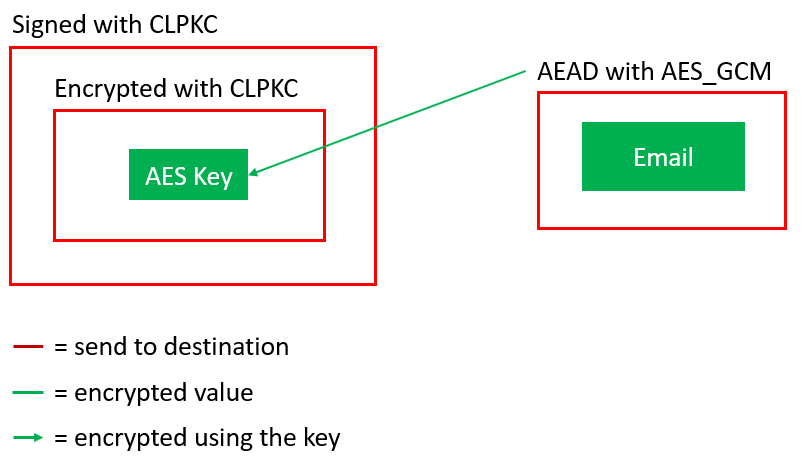
\includegraphics[width=12cm]{images/schemaEncapsulation.png}
	\caption{Schéma encapsulation des données}
	\label{fig:encapsulate}
\end{figure}

\section{Fonctionnement global POC (KGC)}
Ici je présente le fonctionnement global de mon implémentation du KGC pour mon POC. De plus je présente les problèmes connus et des propositions d'améliorations.
\subsection{Fonctionnement}
\subsection{Problèmes connus}
\subsection{Améliorations}
%\inputsourcecode{c}{"source_code/main.c"}{main.c}
%\inputminted[linenos, numbersep=4pt,fontsize=\footnotesize, breaklines=true]{C}{source_code/main.c}
\section{Fonctionnement global POC (Client)}
Ici je présente le fonctionnement global de l'implémentation du client mail pour mon POC, des améliorations possibles et des problèmes connus.
\subsection{Fonctionnement}
\subsection{Problèmes connus}
\subsection{Améliorations}
\paragraph*{Multiples destinataires.}
\section{Comparaisons}
Dans cette section je vais présenter les différents protocoles et implémentations existantes présentées au chapitre \ref{ch:analysis} et les comparer à mon implémentation. Tout d'abord en présentant les différentes propriétés cryptographiques puis les temps d'exécution.

% TODO à analyser et remplir correctement
\subsection{Propriétés cryptographiques}
\begin{table}[h!]
	\centering
	\begin{tabular}{ |p{3cm}||p{3cm}|p{3cm}| }
		\hline
		\multicolumn{3}{|c|}{Comparaisons des propriétés cryptographiques proposées} \\
		\hline
		Implémentations & E2EE & Forward Secrecy\\
		\hline
		CLPKC-POC   & Oui & Oui\\
		PGP & Oui & Non\\
		S/MIME & Oui & Non\\
		\hline
	\end{tabular}
	\caption{Table de comparaison des différentes propriétés cryptographiques }
	\label{table:comparisonProperties}
\end{table}
% TODO si le temps le permet faire des calculs sur les temps de chiffrement / déchiffrement